% TODO Include picture of circuit 3

\FloatBarrier

\begin{figure}[h!]
	\centering
	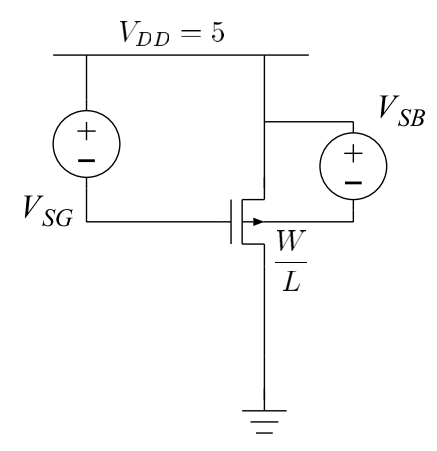
\includegraphics[scale=0.75]{../images/circuit_3.PNG}
	\caption{Circuit 3}
	\label{fig:circuit_3}
\end{figure}

\FloatBarrier

\FloatBarrier

\begin{figure}[h!]
	\centering
	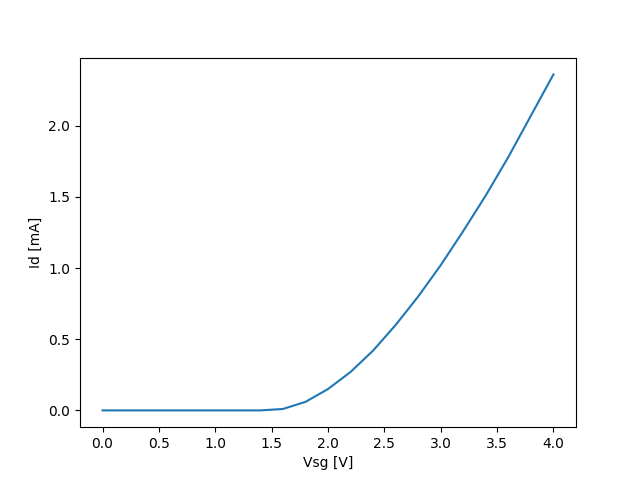
\includegraphics[scale=0.75]{../images/data_3.PNG}
	\caption{$i_{D}$ versus $V_{SG}$ of PMOS where $V_{SB}= 0$\si{\volt}}
	\label{fig:data_3}
\end{figure}

\FloatBarrier

\FloatBarrier

\begin{table}[h!]
	\centering
	\caption{Figure (\ref{fig:data_3}) Data}
	\label{tab:data_3}
	\csvautotabular{../tables/data_3.csv}
\end{table}

\FloatBarrier

As $V_{SG}$ is increased, electrons are repelled from the channel beneath the gate of the PMOS.
This exposes a depletion layer in the channel.
Once $V_{SG}$ hits the threshold voltage $|V_{tp}|$, for which $|V_{tp}| \approx 1.5$\si{\volt} in this case, holes are ripped from the postiviely-charged donor ions in n-type substrate, and a p-type channel is formed. \\

The transistor exits cutoff past $|V_{tp}|$.
If $V_{SD} > V_{SG} - |V_{tp}|$, then the transistor operates in the saturation region.
The drain in this circuit is grounded.
The source is set to supply, which is $V_{DD} = 5$\si{\volt}.
Therefore, $V_{SD} = 5$\si{\volt}.
If $|V_{tp}| \geq 0$ by the definition of the absolute value of a real number.
Therefore, so long as $V_{SG} < V_{SD} + |V_{tp}| \leq 5$\si{\volt}, the transistor stays in saturation.
If $V_{SG}$ is increased past about $4$\si{\volt}, the current in the actual experiment becomes much too large to handle.
As a result, the test cases are limited to $V_{SG} < 4$\si{\volt}.
Thus, by design, the transistor exits cutoff and enters saturation, in which case the current grows with $V_{SG}^{2}$. \\

\FloatBarrier

\begin{figure}[h!]
	\centering
	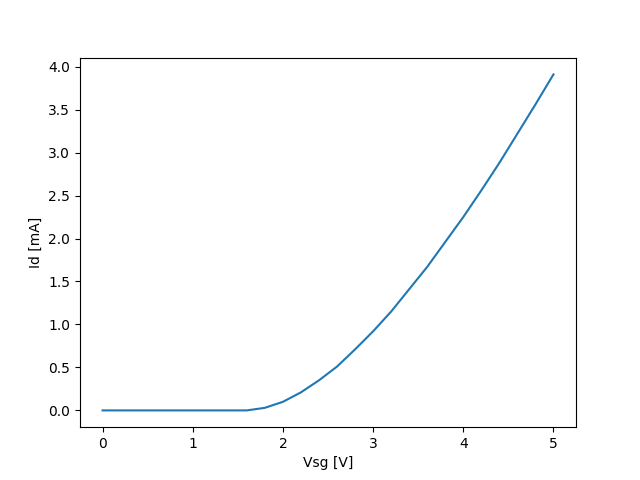
\includegraphics[scale=0.75]{../images/data_3_b.PNG}
	\caption{$i_{D}$ versus $V_{SG}$ of PMOS where $V_{SB}= 0.5$\si{\volt}}
	\label{fig:data_3_b}
\end{figure}

\FloatBarrier

\FloatBarrier

\begin{table}[h!]
	\centering
	\caption{Figure (\ref{fig:data_3_b}) Data}
	\label{tab:data_3_b}
	\csvautotabular{../tables/data_3_b.csv}
\end{table}

\FloatBarrier

When increasing the source-bulk voltage $V_{SB}$, the threshold voltage increases slightly to about $1.7$\si{\volt}.
In a very simplified model, two pn-junction diodes exist in a PMOS transistor.
The first is between the source and the bulk.
The other is between the drain and the bulk.
Initially, the source and bulk voltages are both $5$\si{\volt} relative to ground.
In this situation, because the drain is grounded, a slight reverse saturation current occurs from the bulk to the drain, but no current flows from the source to the bulk.
Now, drop the bulk voltage to $4.5$\si{\volt}, so that $V_{SB} = 0.5$\si{\volt}, while still keeping the source at the supply voltage.
The reverse saturation current in the drain-bulk diode drops slightly, meaning less current flows into the drain.
Moreover, the current from the source to the bulk increases dramatically.
As a result, current is drawn from the source, and less current flows into the drain.
Therefore, less current flows through the channel.
So, a higher $V_{SG}$ is required to achieve the same current.
Thus, the threshold voltage $|V_{tp}|$ must increase.
The transistor exits cutoff around $1.6$\si{\volt} this time.
Therefore, in line with theory, the threshold voltage increased slightly with the increased $V_{SB}$, namely from about $1.5$\si{\volt} to $1.7$\si{\volt}.

% TODO W/L ratio of transistor

The current in the saturation region for an NMOS transistor is approximately given by:

\begin{equation}
	\label{eq:nmos_sat}
	i_{D} = \frac{k_{n}'}{2} \frac{W}{L} ( V_{GS} - V_{tn} )^{2}
\end{equation}

Rearranging the equation, the NMOS's $\frac{W}{L}$ ratio can be determined:

\begin{equation}
	\label{eq:w_over_l_nmos}
	\frac{W}{L} = \frac{2 i_{D}}{k_{n}' (V_{GS} - V_{tn})^{2}}
\end{equation}

A similar result is obtained for the PMOS:

\begin{equation}
	\label{eq:w_over_l_pmos}
	\frac{W}{L} = \frac{ 2 i_{D}}{k_{p}' (V_{SG} - |V_{tp}|)^{2}}
\end{equation}

So, if the various parameters on the right-side of either equation are known for different test cases, then $\frac{W}{L}$ can be calculated for different points, and the average can be taken for a good estimate of the true value.
$i_{D}$ and $V_{SG}$ are trivial since those are essentially directly measured in the experiment.
$V_{tn}$ and $|V_{tp}|$ are given in the SPICE model of the CD4007 transistors, but they do not reflect what is observed in the actual transistors.
However, from analyzing the measured data points, the threshold voltages can be easily obtained for the transistors in lab, and those are to be used.
The threshold voltages are given in table (\ref{tab:vt}):

\FloatBarrier

\begin{table}[h!]
	\centering
	\caption{Measured Threshold Voltages for NMOS and PMOS}
	\label{tab:vt}
	\csvautotabular{../tables/vt.csv}
\end{table}

\FloatBarrier

The only unknown values are the process transconductance parameters $k_{n}'$ and $k_{p}'$.
It is difficult to decouple $k_{n}'$ from $\frac{W}{L}$.
The same applies to the PMOS values.
So, the $k_{n}'$ and $k_{p}'$ values from the SPICE model are to be used.

\FloatBarrier

\begin{table}[h!]
	\centering
	\caption{SPICE Model Process Transconductance Parameters for NMOS and PMOS}
	\label{tab:k}
	\csvautotabular{../tables/k.csv}
\end{table}

\FloatBarrier

Using the data in tables (\ref{tab:vt}) and (\ref{tab:k}) as well as equations (\ref{eq:w_over_l_nmos}) and (\ref{eq:w_over_l_pmos}), the $\frac{W}{L}$ ratios for each transistor can be approximated.

\FloatBarrier

\begin{table}[h!]
	\centering
	\caption{$\frac{W}{L}$ Ratios for NMOS and PMOS}
	\label{tab:w_over_l}
	\csvautotabular{../tables/w_over_l.csv}
\end{table}

\FloatBarrier
